\documentclass[12pt]{article}

%packages
%\usepackage{latexsym}
\usepackage{graphicx}
\usepackage{color}
\usepackage{amsmath}
%\usepackage{dsfont}
\usepackage{placeins}
\usepackage{amssymb}
\usepackage{wasysym}
\usepackage{abstract}
\usepackage{hyperref}

%\usepackage{pstricks,pst-node,pst-tree}

%\usepackage{algpseudocode}
%\usepackage{amsthm}
%\usepackage{hyperref}
%\usepackage{mathrsfs}
%\usepackage{amsfonts}
%\usepackage{bbding}
%\usepackage{listings}
%\usepackage{appendix}
\usepackage[margin=1in]{geometry}
%\geometry{papersize={8.5in,11in},total={6.5in,9in}}
%\usepackage{cancel}
%\usepackage{algorithmic, algorithm}

\newcounter{probnum}
\setcounter{probnum}{1}

%create definition to allow local margin changes
\def\changemargin#1#2{\list{}{\rightmargin#2\leftmargin#1}\item[]}
\let\endchangemargin=\endlist 

%allow equations to span multiple pages
\allowdisplaybreaks

%define colors and color typesetting conveniences
\definecolor{gray}{rgb}{0.5,0.5,0.5}
\definecolor{black}{rgb}{0,0,0}
\definecolor{white}{rgb}{1,1,1}
\definecolor{blue}{rgb}{0.5,0.5,1}
\newcommand{\inblue}[1]{\color{blue}#1 \color{black}}
\definecolor{green}{rgb}{0.133,0.545,0.133}
\newcommand{\ingreen}[1]{\color{green}#1 \color{black}}
\definecolor{yellow}{rgb}{1,0.549,0}
\newcommand{\inyellow}[1]{\color{yellow}#1 \color{black}}
\definecolor{red}{rgb}{1,0.133,0.133}
\newcommand{\inred}[1]{\color{red}#1 \color{black}}
\definecolor{purple}{rgb}{0.58,0,0.827}
\newcommand{\inpurple}[1]{\color{purple}#1 \color{black}}
\definecolor{backgcode}{rgb}{0.97,0.97,0.8}
\definecolor{Brown}{cmyk}{0,0.81,1,0.60}
\definecolor{OliveGreen}{cmyk}{0.64,0,0.95,0.40}
\definecolor{CadetBlue}{cmyk}{0.62,0.57,0.23,0}

%define new math operators
\DeclareMathOperator*{\argmax}{arg\,max~}
\DeclareMathOperator*{\argmin}{arg\,min~}
\DeclareMathOperator*{\argsup}{arg\,sup~}
\DeclareMathOperator*{\arginf}{arg\,inf~}
\DeclareMathOperator*{\convolution}{\text{\Huge{$\ast$}}}
\newcommand{\infconv}[2]{\convolution^\infty_{#1 = 1} #2}
%true functions

%%%% GENERAL SHORTCUTS

%shortcuts for pure typesetting conveniences
\newcommand{\bv}[1]{\boldsymbol{#1}}

%shortcuts for compound constants
\newcommand{\BetaDistrConst}{\dfrac{\Gamma(\alpha + \beta)}{\Gamma(\alpha)\Gamma(\beta)}}
\newcommand{\NormDistrConst}{\dfrac{1}{\sqrt{2\pi\sigma^2}}}

%shortcuts for conventional symbols
\newcommand{\tsq}{\tau^2}
\newcommand{\tsqh}{\hat{\tau}^2}
\newcommand{\sigsq}{\sigma^2}
\newcommand{\sigsqsq}{\parens{\sigma^2}^2}
\newcommand{\sigsqovern}{\dfrac{\sigsq}{n}}
\newcommand{\tausq}{\tau^2}
\newcommand{\tausqalpha}{\tau^2_\alpha}
\newcommand{\tausqbeta}{\tau^2_\beta}
\newcommand{\tausqsigma}{\tau^2_\sigma}
\newcommand{\betasq}{\beta^2}
\newcommand{\sigsqvec}{\bv{\sigma}^2}
\newcommand{\sigsqhat}{\hat{\sigma}^2}
\newcommand{\sigsqhatmlebayes}{\sigsqhat_{\text{Bayes, MLE}}}
\newcommand{\sigsqhatmle}[1]{\sigsqhat_{#1, \text{MLE}}}
\newcommand{\bSigma}{\bv{\Sigma}}
\newcommand{\bSigmainv}{\bSigma^{-1}}
\newcommand{\thetavec}{\bv{\theta}}
\newcommand{\thetahat}{\hat{\theta}}
\newcommand{\thetahatmle}{\hat{\theta}_{\mathrm{MLE}}}
\newcommand{\thetavechatmle}{\hat{\thetavec}_{\mathrm{MLE}}}
\newcommand{\muhat}{\hat{\mu}}
\newcommand{\musq}{\mu^2}
\newcommand{\muvec}{\bv{\mu}}
\newcommand{\muhatmle}{\muhat_{\text{MLE}}}
\newcommand{\lambdahat}{\hat{\lambda}}
\newcommand{\lambdahatmle}{\lambdahat_{\text{MLE}}}
\newcommand{\etavec}{\bv{\eta}}
\newcommand{\alphavec}{\bv{\alpha}}
\newcommand{\minimaxdec}{\delta^*_{\mathrm{mm}}}
\newcommand{\ybar}{\bar{y}}
\newcommand{\xbar}{\bar{x}}
\newcommand{\Xbar}{\bar{X}}
\newcommand{\iid}{~{\buildrel iid \over \sim}~}
\newcommand{\inddist}{~{\buildrel ind \over \sim}~}
\newcommand{\approxdist}{~{\buildrel approx \over \sim}~}
\newcommand{\equalsindist}{~{\buildrel d \over =}~}
\newcommand{\loglik}[1]{\ell\parens{#1}}
\newcommand{\thetahatkminone}{\thetahat^{(k-1)}}
\newcommand{\thetahatkplusone}{\thetahat^{(k+1)}}
\newcommand{\thetahatk}{\thetahat^{(k)}}
\newcommand{\half}{\frac{1}{2}}
\newcommand{\third}{\frac{1}{3}}
\newcommand{\twothirds}{\frac{2}{3}}
\newcommand{\fourth}{\frac{1}{4}}
\newcommand{\fifth}{\frac{1}{5}}
\newcommand{\sixth}{\frac{1}{6}}

%shortcuts for vector and matrix notation
\newcommand{\A}{\bv{A}}
\newcommand{\At}{\A^T}
\newcommand{\Ainv}{\inverse{\A}}
\newcommand{\B}{\bv{B}}
\newcommand{\K}{\bv{K}}
\newcommand{\Kt}{\K^T}
\newcommand{\Kinv}{\inverse{K}}
\newcommand{\Kinvt}{(\Kinv)^T}
\newcommand{\M}{\bv{M}}
\newcommand{\Bt}{\B^T}
\newcommand{\Q}{\bv{Q}}
\newcommand{\Qt}{\Q^T}
\newcommand{\R}{\bv{R}}
\newcommand{\Rt}{\R^T}
\newcommand{\Z}{\bv{Z}}
\newcommand{\X}{\bv{X}}
\newcommand{\Xsub}{\X_{\text{(sub)}}}
\newcommand{\Xsubadj}{\X_{\text{(sub,adj)}}}
\newcommand{\I}{\bv{I}}
\newcommand{\Y}{\bv{Y}}
\newcommand{\sigsqI}{\sigsq\I}
\renewcommand{\P}{\bv{P}}
\newcommand{\Psub}{\P_{\text{(sub)}}}
\newcommand{\Pt}{\P^T}
\newcommand{\Pii}{P_{ii}}
\newcommand{\Pij}{P_{ij}}
\newcommand{\IminP}{(\I-\P)}
\newcommand{\Xt}{\bv{X}^T}
\newcommand{\XtX}{\Xt\X}
\newcommand{\XtXinv}{\parens{\Xt\X}^{-1}}
\newcommand{\XtXinvXt}{\XtXinv\Xt}
\newcommand{\XXtXinvXt}{\X\XtXinvXt}
\newcommand{\x}{\bv{x}}
\newcommand{\onevec}{\bv{1}}
\newcommand{\oneton}{1, \ldots, n}
\newcommand{\yoneton}{y_1, \ldots, y_n}
\newcommand{\yonetonorder}{y_{(1)}, \ldots, y_{(n)}}
\newcommand{\Yoneton}{Y_1, \ldots, Y_n}
\newcommand{\iinoneton}{i \in \braces{\oneton}}
\newcommand{\onetom}{1, \ldots, m}
\newcommand{\jinonetom}{j \in \braces{\onetom}}
\newcommand{\xoneton}{x_1, \ldots, x_n}
\newcommand{\Xoneton}{X_1, \ldots, X_n}
\newcommand{\xt}{\x^T}
\newcommand{\y}{\bv{y}}
\newcommand{\yt}{\y^T}
\renewcommand{\c}{\bv{c}}
\newcommand{\ct}{\c^T}
\newcommand{\tstar}{\bv{t}^*}
\renewcommand{\u}{\bv{u}}
\renewcommand{\v}{\bv{v}}
\renewcommand{\a}{\bv{a}}
\newcommand{\s}{\bv{s}}
\newcommand{\yadj}{\y_{\text{(adj)}}}
\newcommand{\xjadj}{\x_{j\text{(adj)}}}
\newcommand{\xjadjM}{\x_{j \perp M}}
\newcommand{\yhat}{\hat{\y}}
\newcommand{\yhatsub}{\yhat_{\text{(sub)}}}
\newcommand{\yhatstar}{\yhat^*}
\newcommand{\yhatstarnew}{\yhatstar_{\text{new}}}
\newcommand{\z}{\bv{z}}
\newcommand{\zt}{\z^T}
\newcommand{\bb}{\bv{b}}
\newcommand{\bbt}{\bb^T}
\newcommand{\bbeta}{\bv{\beta}}
\newcommand{\beps}{\bv{\epsilon}}
\newcommand{\bepst}{\beps^T}
\newcommand{\e}{\bv{e}}
\newcommand{\Mofy}{\M(\y)}
\newcommand{\KofAlpha}{K(\alpha)}
\newcommand{\ellset}{\mathcal{L}}
\newcommand{\oneminalph}{1-\alpha}
\newcommand{\SSE}{\text{SSE}}
\newcommand{\SSEsub}{\text{SSE}_{\text{(sub)}}}
\newcommand{\MSE}{\text{MSE}}
\newcommand{\RMSE}{\text{RMSE}}
\newcommand{\SSR}{\text{SSR}}
\newcommand{\SST}{\text{SST}}
\newcommand{\JSest}{\delta_{\text{JS}}(\x)}
\newcommand{\Bayesest}{\delta_{\text{Bayes}}(\x)}
\newcommand{\EmpBayesest}{\delta_{\text{EmpBayes}}(\x)}
\newcommand{\BLUPest}{\delta_{\text{BLUP}}}
\newcommand{\MLEest}[1]{\hat{#1}_{\text{MLE}}}

%shortcuts for Linear Algebra stuff (i.e. vectors and matrices)
\newcommand{\twovec}[2]{\bracks{\begin{array}{c} #1 \\ #2 \end{array}}}
\newcommand{\threevec}[3]{\bracks{\begin{array}{c} #1 \\ #2 \\ #3 \end{array}}}
\newcommand{\fivevec}[5]{\bracks{\begin{array}{c} #1 \\ #2 \\ #3 \\ #4 \\ #5 \end{array}}}
\newcommand{\twobytwomat}[4]{\bracks{\begin{array}{cc} #1 & #2 \\ #3 & #4 \end{array}}}
\newcommand{\threebytwomat}[6]{\bracks{\begin{array}{cc} #1 & #2 \\ #3 & #4 \\ #5 & #6 \end{array}}}

%shortcuts for conventional compound symbols
\newcommand{\thetainthetas}{\theta \in \Theta}
\newcommand{\reals}{\mathbb{R}}
\newcommand{\complexes}{\mathbb{C}}
\newcommand{\rationals}{\mathbb{Q}}
\newcommand{\integers}{\mathbb{Z}}
\newcommand{\naturals}{\mathbb{N}}
\newcommand{\forallninN}{~~\forall n \in \naturals}
\newcommand{\forallxinN}[1]{~~\forall #1 \in \reals}
\newcommand{\matrixdims}[2]{\in \reals^{\,#1 \times #2}}
\newcommand{\inRn}[1]{\in \reals^{\,#1}}
\newcommand{\mathimplies}{\quad\Rightarrow\quad}
\newcommand{\mathlogicequiv}{\quad\Leftrightarrow\quad}
\newcommand{\eqncomment}[1]{\quad \text{(#1)}}
\newcommand{\limitn}{\lim_{n \rightarrow \infty}}
\newcommand{\limitN}{\lim_{N \rightarrow \infty}}
\newcommand{\limitd}{\lim_{d \rightarrow \infty}}
\newcommand{\limitt}{\lim_{t \rightarrow \infty}}
\newcommand{\limitsupn}{\limsup_{n \rightarrow \infty}~}
\newcommand{\limitinfn}{\liminf_{n \rightarrow \infty}~}
\newcommand{\limitk}{\lim_{k \rightarrow \infty}}
\newcommand{\limsupn}{\limsup_{n \rightarrow \infty}}
\newcommand{\limsupk}{\limsup_{k \rightarrow \infty}}
\newcommand{\floor}[1]{\left\lfloor #1 \right\rfloor}
\newcommand{\ceil}[1]{\left\lceil #1 \right\rceil}

%shortcuts for environments
\newcommand{\beqn}{\vspace{-0.25cm}\begin{eqnarray*}}
\newcommand{\eeqn}{\end{eqnarray*}}
\newcommand{\bneqn}{\vspace{-0.25cm}\begin{eqnarray}}
\newcommand{\eneqn}{\end{eqnarray}}

%shortcuts for mini environments
\newcommand{\parens}[1]{\left(#1\right)}
\newcommand{\squared}[1]{\parens{#1}^2}
\newcommand{\tothepow}[2]{\parens{#1}^{#2}}
\newcommand{\prob}[1]{\mathbb{P}\parens{#1}}
\newcommand{\littleo}[1]{o\parens{#1}}
\newcommand{\bigo}[1]{O\parens{#1}}
\newcommand{\Lp}[1]{\mathbb{L}^{#1}}
\renewcommand{\arcsin}[1]{\text{arcsin}\parens{#1}}
\newcommand{\prodonen}[2]{\bracks{\prod_{#1=1}^n #2}}
\newcommand{\mysum}[4]{\sum_{#1=#2}^{#3} #4}
\newcommand{\sumonen}[2]{\sum_{#1=1}^n #2}
\newcommand{\infsum}[2]{\sum_{#1=1}^\infty #2}
\newcommand{\infprod}[2]{\prod_{#1=1}^\infty #2}
\newcommand{\infunion}[2]{\bigcup_{#1=1}^\infty #2}
\newcommand{\infinter}[2]{\bigcap_{#1=1}^\infty #2}
\newcommand{\infintegral}[2]{\int^\infty_{-\infty} #2 ~\text{d}#1}
\newcommand{\supthetas}[1]{\sup_{\thetainthetas}\braces{#1}}
\newcommand{\bracks}[1]{\left[#1\right]}
\newcommand{\braces}[1]{\left\{#1\right\}}
\newcommand{\set}[1]{\left\{#1\right\}}
\newcommand{\abss}[1]{\left|#1\right|}
\newcommand{\norm}[1]{\left|\left|#1\right|\right|}
\newcommand{\normsq}[1]{\norm{#1}^2}
\newcommand{\inverse}[1]{\parens{#1}^{-1}}
\newcommand{\rowof}[2]{\parens{#1}_{#2\cdot}}

%shortcuts for functionals
\newcommand{\realcomp}[1]{\text{Re}\bracks{#1}}
\newcommand{\imagcomp}[1]{\text{Im}\bracks{#1}}
\newcommand{\range}[1]{\text{range}\bracks{#1}}
\newcommand{\colsp}[1]{\text{colsp}\bracks{#1}}
\newcommand{\rowsp}[1]{\text{rowsp}\bracks{#1}}
\newcommand{\tr}[1]{\text{tr}\bracks{#1}}
\newcommand{\rank}[1]{\text{rank}\bracks{#1}}
\newcommand{\proj}[2]{\text{Proj}_{#1}\bracks{#2}}
\newcommand{\projcolspX}[1]{\text{Proj}_{\colsp{\X}}\bracks{#1}}
\newcommand{\median}[1]{\text{median}\bracks{#1}}
\newcommand{\mean}[1]{\text{mean}\bracks{#1}}
\newcommand{\dime}[1]{\text{dim}\bracks{#1}}
\renewcommand{\det}[1]{\text{det}\bracks{#1}}
\newcommand{\expe}[1]{\mathbb{E}\bracks{#1}}
\newcommand{\expeabs}[1]{\expe{\abss{#1}}}
\newcommand{\expesub}[2]{\mathbb{E}_{#1}\bracks{#2}}
\newcommand{\indic}[1]{\mathds{1}_{#1}}
\newcommand{\var}[1]{\mathbb{V}\text{ar}\bracks{#1}}
\newcommand{\sd}[1]{\mathbb{S}\text{D}\bracks{#1}}
\newcommand{\cov}[2]{\text{Cov}\bracks{#1, #2}}
\newcommand{\corr}[2]{\text{Corr}\bracks{#1, #2}}
\newcommand{\se}[1]{\text{SE}\bracks{#1}}
\newcommand{\seest}[1]{\hat{\text{SE}}\bracks{#1}}
\newcommand{\bias}[1]{\text{Bias}\bracks{#1}}
\newcommand{\partialop}[2]{\dfrac{\partial}{\partial #1}\bracks{#2}}
\newcommand{\secpartialop}[2]{\dfrac{\partial^2}{\partial #1^2}\bracks{#2}}
\newcommand{\mixpartialop}[3]{\dfrac{\partial^2}{\partial #1 \partial #2}\bracks{#3}}

%shortcuts for functions
\renewcommand{\exp}[1]{\mathrm{exp}\parens{#1}}
\renewcommand{\cos}[1]{\text{cos}\parens{#1}}
\renewcommand{\sin}[1]{\text{sin}\parens{#1}}
\newcommand{\sign}[1]{\text{sign}\parens{#1}}
\newcommand{\are}[1]{\mathrm{ARE}\parens{#1}}
\newcommand{\natlog}[1]{\ln\parens{#1}}
\newcommand{\oneover}[1]{\frac{1}{#1}}
\newcommand{\overtwo}[1]{\frac{#1}{2}}
\newcommand{\overn}[1]{\frac{#1}{n}}
\newcommand{\oneoversqrt}[1]{\oneover{\sqrt{#1}}}
\newcommand{\sqd}[1]{\parens{#1}^2}
\newcommand{\loss}[1]{\ell\parens{\theta, #1}}
\newcommand{\losstwo}[2]{\ell\parens{#1, #2}}
\newcommand{\cf}{\phi(t)}

%English language specific shortcuts
\newcommand{\ie}{\textit{i.e.} }
\newcommand{\AKA}{\textit{AKA} }
\renewcommand{\iff}{\textit{iff}}
\newcommand{\eg}{\textit{e.g.} }
\newcommand{\st}{\textit{s.t.} }
\newcommand{\wrt}{\textit{w.r.t.} }
\newcommand{\mathst}{~~\text{\st}~~}
\newcommand{\mathand}{~~\text{and}~~}
\newcommand{\ala}{\textit{a la} }
\newcommand{\ppp}{posterior predictive p-value}
\newcommand{\dd}{dataset-to-dataset}

%shortcuts for distribution titles
\newcommand{\logistic}[2]{\mathrm{Logistic}\parens{#1,\,#2}}
\newcommand{\bernoulli}[1]{\mathrm{Bernoulli}\parens{#1}}
\newcommand{\betanot}[2]{\mathrm{Beta}\parens{#1,\,#2}}
\newcommand{\stdbetanot}{\betanot{\alpha}{\beta}}
\newcommand{\multnormnot}[3]{\mathcal{N}_{#1}\parens{#2,\,#3}}
\newcommand{\normnot}[2]{\mathcal{N}\parens{#1,\,#2}}
\newcommand{\classicnormnot}{\normnot{\mu}{\sigsq}}
\newcommand{\stdnormnot}{\normnot{0}{1}}
\newcommand{\uniform}[2]{\mathrm{U}\parens{#1,\,#2}}
\newcommand{\stduniform}{\uniform{0}{1}}
\newcommand{\exponential}[1]{\mathrm{Exp}\parens{#1}}
\newcommand{\gammadist}[2]{\mathrm{Gamma}\parens{#1, #2}}
\newcommand{\poisson}[1]{\mathrm{Poisson}\parens{#1}}
\newcommand{\binomial}[2]{\mathrm{Binomial}\parens{#1,\,#2}}
\newcommand{\rayleigh}[1]{\mathrm{Rayleigh}\parens{#1}}
\newcommand{\multinomial}[2]{\mathrm{Multinomial}\parens{#1,\,#2}}
\newcommand{\gammanot}[2]{\mathrm{Gamma}\parens{#1,\,#2}}
\newcommand{\cauchynot}[2]{\text{Cauchy}\parens{#1,\,#2}}
\newcommand{\invchisqnot}[1]{\text{Inv}\chisq{#1}}
\newcommand{\invscaledchisqnot}[2]{\text{ScaledInv}\ncchisq{#1}{#2}}
\newcommand{\invgammanot}[2]{\text{InvGamma}\parens{#1,\,#2}}
\newcommand{\chisq}[1]{\chi^2_{#1}}
\newcommand{\ncchisq}[2]{\chi^2_{#1}\parens{#2}}
\newcommand{\ncF}[3]{F_{#1,#2}\parens{#3}}

%shortcuts for PDF's of common distributions
\newcommand{\logisticpdf}[3]{\oneover{#3}\dfrac{\exp{-\dfrac{#1 - #2}{#3}}}{\parens{1+\exp{-\dfrac{#1 - #2}{#3}}}^2}}
\newcommand{\betapdf}[3]{\dfrac{\Gamma(#2 + #3)}{\Gamma(#2)\Gamma(#3)}#1^{#2-1} (1-#1)^{#3-1}}
\newcommand{\normpdf}[3]{\frac{1}{\sqrt{2\pi#3}}\exp{-\frac{1}{2#3}(#1 - #2)^2}}
\newcommand{\normpdfvarone}[2]{\dfrac{1}{\sqrt{2\pi}}e^{-\half(#1 - #2)^2}}
\newcommand{\chisqpdf}[2]{\dfrac{1}{2^{#2/2}\Gamma(#2/2)}\; {#1}^{#2/2-1} e^{-#1/2}}
\newcommand{\invchisqpdf}[2]{\dfrac{2^{-\overtwo{#1}}}{\Gamma(#2/2)}\,{#1}^{-\overtwo{#2}-1}  e^{-\oneover{2 #1}}}
\newcommand{\exponentialpdf}[2]{#2\exp{-#2#1}}
\newcommand{\poissonpdf}[2]{\dfrac{e^{-#1} #1^{#2}}{#2!}}
\newcommand{\binomialpdf}[3]{\binom{#2}{#1}#3^{#1}(1-#3)^{#2-#1}}
\newcommand{\rayleighpdf}[2]{\dfrac{#1}{#2^2}\exp{-\dfrac{#1^2}{2 #2^2}}}
\newcommand{\gammapdf}[3]{\dfrac{#3^#2}{\Gamma\parens{#2}}#1^{#2-1}\exp{-#3 #1}}
\newcommand{\cauchypdf}[3]{\oneover{\pi} \dfrac{#3}{\parens{#1-#2}^2 + #3^2}}
\newcommand{\Gammaf}[1]{\Gamma\parens{#1}}

%shortcuts for miscellaneous typesetting conveniences
\newcommand{\notesref}[1]{\marginpar{\color{gray}\tt #1\color{black}}}

%%%% DOMAIN-SPECIFIC SHORTCUTS

%Real analysis related shortcuts
\newcommand{\zeroonecl}{\bracks{0,1}}
\newcommand{\forallepsgrzero}{\forall \epsilon > 0~~}
\newcommand{\lessthaneps}{< \epsilon}
\newcommand{\fraccomp}[1]{\text{frac}\bracks{#1}}

%Bayesian related shortcuts
\newcommand{\yrep}{y^{\text{rep}}}
\newcommand{\yrepisq}{(\yrep_i)^2}
\newcommand{\yrepvec}{\bv{y}^{\text{rep}}}


%Probability shortcuts
\newcommand{\SigField}{\mathcal{F}}
\newcommand{\ProbMap}{\mathcal{P}}
\newcommand{\probtrinity}{\parens{\Omega, \SigField, \ProbMap}}
\newcommand{\convp}{~{\buildrel p \over \rightarrow}~}
\newcommand{\convLp}[1]{~{\buildrel \Lp{#1} \over \rightarrow}~}
\newcommand{\nconvp}{~{\buildrel p \over \nrightarrow}~}
\newcommand{\convae}{~{\buildrel a.e. \over \longrightarrow}~}
\newcommand{\convau}{~{\buildrel a.u. \over \longrightarrow}~}
\newcommand{\nconvau}{~{\buildrel a.u. \over \nrightarrow}~}
\newcommand{\nconvae}{~{\buildrel a.e. \over \nrightarrow}~}
\newcommand{\convd}{~{\buildrel \mathcal{D} \over \rightarrow}~}
\newcommand{\nconvd}{~{\buildrel \mathcal{D} \over \nrightarrow}~}
\newcommand{\withprob}{~~\text{w.p.}~~}
\newcommand{\io}{~~\text{i.o.}}

\newcommand{\Acl}{\bar{A}}
\newcommand{\ENcl}{\bar{E}_N}
\newcommand{\diam}[1]{\text{diam}\parens{#1}}

\newcommand{\taua}{\tau_a}

\newcommand{\myint}[4]{\int_{#2}^{#3} #4 \,\text{d}#1}
\newcommand{\laplacet}[1]{\mathscr{L}\bracks{#1}}
\newcommand{\laplaceinvt}[1]{\mathscr{L}^{-1}\bracks{#1}}
\renewcommand{\min}[1]{\text{min}\braces{#1}}

\newcommand{\Vbar}[1]{\bar{V}\parens{#1}}
\newcommand{\expnegrtau}{\exp{-r\tau}}

%%% problem typesetting
\newcommand{\problem}{\vspace{0.2cm} \noindent {\large{\textsf{Problem \arabic{probnum}~}}} \addtocounter{probnum}{1}}
%\newcommand{\easyproblem}{\ingreen{\noindent \textsf{Problem \arabic{probnum}~}} \addtocounter{probnum}{1}}
%\newcommand{\intermediateproblem}{\noindent \inyellow{\textsf{Problem \arabic{probnum}~}} \addtocounter{probnum}{1}}
%\newcommand{\hardproblem}{\inred{\noindent \textsf{Problem \arabic{probnum}~}} \addtocounter{probnum}{1}}
%\newcommand{\extracreditproblem}{\noindent \inpurple{\textsf{Problem \arabic{probnum}~}} \addtocounter{probnum}{1}}

\newcommand{\easysubproblem}{\ingreen{\item}}
\newcommand{\intermediatesubproblem}{\inyellow{\item}}
\newcommand{\hardsubproblem}{\inred{\item}}
\newcommand{\extracreditsubproblem}{\inpurple{\item}}
\renewcommand{\labelenumi}{(\alph{enumi})}


\title{Statistics 101 Summer I 2011 \\ Homework \#3}
\author{Adam Kapelner, Instructor}

\date{Due noon, Friday, June 17, 2011 (in my mail slot)}

\renewcommand{\abstractname}{Instructions and Philosophy}

\begin{document}
\maketitle


\begin{abstract}
Copy paragraph one from last week's introduction about working hard on problems and working in teams.

In Stine \& Foster, read chapter 4 over including the last section on the empirical rule, read chapter 13 on surveys and sampling, read chapter 12 on continuous r.v.'s and the central limit theorem, then chapter 14 on basic applications including control limits. You can ignore the subsection on skewness and kurtosis (pp 275-276) and the subsection on ``sample size condition'' to test for normality (pp 328-329). Also, read the first few pages of chapter 15.

Once again, \ingreen{green} means \textit{easy}, \inyellow{yellow} means \textit{intermediate}, \inred{red} means \textit{difficult}, and \inpurple{purple} means \textit{extra credit}. This homework is worth 100 points but the point distribution will not be determined until after the due date. Late homework will be penalized 10 points per day. Beyond Friday June 17 at 5PM, it will receive a zero. 15 points are given as a bonus if the homework is typed using \LaTeX ~(please comment out or delete all extraneous text).
\end{abstract}


\paragraph{Basic Data Analysis and Sampling} This section will cover the nitty-gritty of data tables, summary statistics, and sampling / surveys. \\

\problem This is a simple data problem. The ages of 25 billionaires living in NY today are 66, 92, 54, 86, 59, 79, 64, 78, 60, 73, 34, 42, 85, 77, 90, 64, 64, 64, 78, 58, 48, 78, 81, 72, 66.

\benum
\easysubproblem Find the average and sample standard deviation with JMP.\footnote{This part was originally assigned without JMP, but now that we've had the midterm, you can use JMP only if you know the formulas well, otherwise I recommend doing it from scratch so you learn how to to do it well.} Indicate units.
\easysubproblem Estimate the mean and standard deviation for all billionaires in NY.
\easysubproblem In the previous question, are we allowed to do that? Explain. 
\easysubproblem Find the five-number summary, IQR, and range.
\easysubproblem Without doing the next parts of the question, evaluate whether or not there is a skew.
\easysubproblem If there is a skew, what methods would you use to fix the skew? Does the transformation make sense?
\easysubproblem Find the median of the transformed data set. Indicate how you would find the mean but do not calculate it.
\easysubproblem How will the median and mean change if the youngest and oldest billionaires in the sample
moved out of NY?
\easysubproblem Construct a histogram with bin width = 5 by hand
\intermediatesubproblem Construct a box and whisker plot by hand above the histogram. Add dots for outliers if they exist. For the half-width of the diamond, use 7. We will be learning how to calculate this half-width next week.
\easysubproblem Could we use the empirical rule to estimate the amount of data between sd's?
\eenum

\problem This problem is to be done without the use of JMP. Table \ref{tab:kapcha_data} is an excerpt of real data from a \href{http://www.mendeley.com/download/public/876311/3709908162/db46ccaeedcab59e40e61cf50e72b6b4d5b8dcdd/dl.pdf}{study} I did with a collaborator at MIT about online survey presentation.\footnote{If you care more, click \href{http://www.crowdconf2010.com/fundamental.html}{here} to watch us embarass ourselves in San Francisco (minute 7:35).}

\begin{table}[htp]
\centering
\footnotesize
\begin{tabular}{c|c|c|c|c|c}
id	& treatment &	created at date	& created at time & amount qu 1 & \# switches \\
\hline
1147	&kapcha	&9/1/2010	&13:33:42	&1.75	&2 \\																						
1150	&timing	&9/1/2010	&13:33:43	&3	&194 \\																						
1152	&timing	&9/1/2010	&14:00:08	&1.5	&8 \\																						
1153	&kapcha	&9/1/2010	&14:00:08	&5	&200 \\																						
1154	&kapcha	&9/1/2010	&14:00:08	&1.5	&31 \\																						
1157	&control	&9/1/2010	&14:00:10	&1	&32 \\																						
1158	&exhortation	&9/1/2010	&14:00:10	&2	&32 \\																						
1159	&kapcha	&9/1/2010	&14:00:10	&1.29	&40 \\																						
1160	&exhortation	&9/1/2010	&14:00:11	&2	&196 \\																						
1161	&timing	&9/1/2010	&14:00:11	&1.5	&214 \\																						
1162	&exhortation	&9/1/2010	&14:00:12	&1	&200 \\																						
1163	&kapcha	&9/1/2010	&14:00:12	&1.5	&208 \\																					
1170	&control	&9/1/2010	&14:00:15	&1.5	&32 \\																						
1171	&kapcha	&9/1/2010	&14:00:15	&2	&36 \\																						
1173	&control	&9/1/2010	&14:00:16	&1.25	&196 \\																						
1178	&control	&9/1/2010	&14:00:18	&2.5	&195 \\																						
1184	&timing	&9/1/2010	&14:00:20	&1.3	&223 \\																						
1186	&kapcha	&9/1/2010	&14:00:21	&2	&203 \\																						
1187	&exhortation	&9/1/2010	&14:00:22	&2	&199 \\																						
1188	&kapcha	&9/1/2010	&14:00:22	&1	&36 \\																						
1191	&kapcha	&9/1/2010	&14:00:23	&2	&200 \\																						
1192	&timing	&9/1/2010	&14:00:24	&2.5	&190 \\																						
1197	&kapcha	&9/1/2010	&14:00:26	&1	&0 \\																						
1198	&exhortation	&9/1/2010	&14:00:26	&5	&32 \\																						
\end{tabular}
\caption{Data excerpted from the Kapcha study}
\label{tab:kapcha_data}
\end{table}

\benum
\easysubproblem We spoke about different types of variables in class: numeric (either interval or taio) and categorical (either nominal or ordinal). What kind of variable is the ``treatment'' column?
\easysubproblem Create a pie chart for the data in the ``treatment'' column.
\intermediatesubproblem What kind of variable is the ``id'' column? This question is designated \inyellow{intermediate} for a reason.
\intermediatesubproblem The ``created at date'' column is sort of useless. Explain how you would combine the ``created at date'' column and another column to make a more useful variable.
\easysubproblem What type of data is the ``amount qu 1'' column?
\easysubproblem What type of data is the ``\# switches'' column?
\intermediatesubproblem The ``\# switches'' column looks like it's trimodal (\ie has three clusters). This is an example where it may be easier to analyze the data if we convert it to a categorical variable. Let's do this. Name the variable ``switch behavior'' and convert each observation into your new variable.
\easysubproblem What type of variable is the new ``switch behavior'' column?
\intermediatesubproblem Now, create a bar chart for the ``switch behavior'' data. Does the order of the categories on the x-axis matter?
\eenum

\problem This problem will ask questions about sampling theory. This will be the fuzziest section of any homework I will assign. You may want to have the book and your notes handy.

\benum
\easysubproblem Define ``population'' and ``sample'' and their respective sizes using the notation from class.
\intermediatesubproblem Explain why a non-representative sample can be biased and why that would be bad.
\easysubproblem We can use $\xbar$ to estimate $\mu$ and $s^2$ to estimate $\sigsq$ only if the data was sampled using a \_\_\_\_\_. Fill in the blank and explain.
\easysubproblem If your sampling method is non-representative, explain why simply sampling more data won't help you.
\intermediatesubproblem Download the \texttt{cars\_mpg.JMP} file. Use these cars as a sampling frame and sample 30 cars using the method taught in class (p.309 of S\&F). Print out your resulting table and circle the 30 you're choosing.
\intermediatesubproblem Do the same sampling five times and list the five $\xbar$'s for the HWYMPG column for each of the 5 samplings. Why are each of these $\xbar$'s different?
\easysubproblem I am running a survey for my arts and crafts store and I sample 30 customers between the ages of 5-15, 30 customers between the ages of 15-25, 30 customers between the ages of 25-35, 30 customers between the ages of 35-45, 30 customers between the ages of 45-55, 30 customers between the ages of 55-65, and 30 customers between the ages of 65-75. What kind of survey is this? Is it biased? Can the biased be fixed?
\intermediatesubproblem I want to find out about people who use public transportation in Philadelphia so I talk to  people who will talk to me on the 42 bus\footnote{service to Upper Darby via Walnut Street and Spruce Street}. Is this a simple random sample? If not, what did I fail to account for?
\easysubproblem When the United States runs their census every 10 years, what is their sampling goal?
\eenum

\paragraph{Continuous r.v.'s} This section will cover some ideas about continuous r.v.'s as well as the basics of the normal curve. Since we are not focusing on computation, I will expect you to use tools that make the computation trivial, so you can learn the concepts. \\

\problem In this problem we will look at the exponential r.v. below:

\beqn
X \sim \exponential{\lambda} = f_X(x) = \lambda e^{-\lambda x}, \quad x \geq 0
\eeqn

Notice we have one parameter, $\lambda$. Exponential random variables are used to model waiting times. Let's pretend $X$ models the time to wait for a bus in minutes. 



\begin{figure}[htp]
\centering
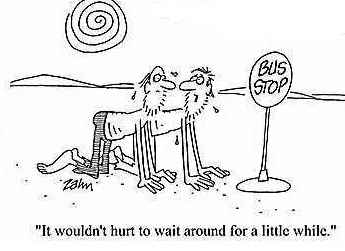
\includegraphics[width=4in, height=2.9in]{busstop.jpg}
\end{figure}
\FloatBarrier

\benum
\easysubproblem To make the case simple, let $\lambda = 0.1$, something we'll relax later. Write the PDF (not PMF, this is a continuous r.v.). Use the $f_X(x)$ notation. Be sure to indicate where $x$ is defined.
\easysubproblem Plot the PDF by sketching it with pencil. Since this is not a calculus class, I recommend using the website \href{http://www.wolframalpha.com}{Wolfram Alpha} (WA). Type in ``\texttt{Plot[0.1 e\textasciicircum\{-0.1 x\}, \{x,0,50\}]}'' into WA and press enter. Copy the plot onto your paper.
\easysubproblem Find the probability that you wait for the bus more than 10 minutes \ie $\prob{X>10}$. On WA, type in ``\texttt{Integrate[0.1 e\textasciicircum\{-0.1 x\}, \{x, 10, Inf\}]}''. Make sure you write the integral you use, then answer as a number.
\easysubproblem Calculate $\expe{X}$ by using ``\texttt{Integrate[x 0.1 e\textasciicircum\{-0.1 x\}, \{x,0,Inf\}]}''.
\intermediatesubproblem Calculate $\expe{X}$ with $\lambda$ as an indeterminate parameter. This will require you to use WA a little more creatively.\footnote{Don't be confused by the output ``Re($\cdot$)''. This is WA making sure whatever your parameter variable you chose is a real number, which it is for the real case of waiting for a bus.}
\extracreditsubproblem Let's say you've been at the busstop for 10min already. What's the probability that you wait more than 10 minutes more? Compare with part (c). Does that make sense? Is the bus tricking you? Explain why the exponential r.v. is called the ``memoryless'' r.v.
\eenum

\problem We will practice using the normal table in this example. Please \textit{draw a picture} and shade in the relevant areas for parts a---f. We assume the standard notation that $Z \sim \stdnormnot$. Find...

\benum
\easysubproblem $\prob{Z < 1.8}$
\easysubproblem $\prob{Z \leq 1.8}$
\easysubproblem $\prob{Z \leq -1.8}$
\easysubproblem $\prob{|Z| \leq 1.8}$
\easysubproblem $\prob{|Z| \geq 1.8}$
\hardsubproblem $\prob{Z \in [-1.5, -1.2] \cup Z \in [1.2,1.5]}$
\easysubproblem the $z$ such that $\prob{Z < z} = 0.99$
\easysubproblem the $z$ such that $\prob{Z < z} = 0.95$
\easysubproblem the $z$ such that $\prob{Z < z} = 0.68$
\easysubproblem $z_{0.0015}$ \ie find the $z$ such that $\prob{|Z| < z} = 0.997$
\easysubproblem $z_{0.025}$ \ie find the $z$ such that $\prob{|Z| < z} = 0.95$
\easysubproblem $z_{0.16}$ \ie find the $z$ such that $\prob{|Z| < z} = 0.68$
\easysubproblem What are the $z$ values to keep in mind for the \textit{empirical rule} (p.65)? Refer to the last six subparts and the find the three we are looking for.
\eenum

\problem We will practice shifts and scales. Consider the following:

\beqn
X \sim \normnot{\mu}{\sigsq} \quad \text{and now we create a transformation:} \quad Z = \frac{X-\mu}{\sigma}
\eeqn

\benum
\easysubproblem What is $\expe{X}$ and $\sd{X}$? This is training you to understand the notation.
\easysubproblem What is the transformation into $Z$ called? Why do we use that name?
\easysubproblem Find $\expe{Z}$ using the formulas from chapter 9.
\easysubproblem Find $\sd{Z}$ using the formulas from chapter 9.
\hardsubproblem Graph all three of the following r.v.'s to scale on the same axis and label $f_{X_1}(x), f_{X_2}(x)$, and $f_{X_3}(x)$:

\beqn
X_1 \sim \normnot{-3}{1^2}, \quad X_2 \sim \normnot{4}{2^2}, \quad X_3 \sim \normnot{1}{\squared{\tenth}}
\eeqn


\textbf{Rule of thumb}: by $\pm 3$ sd's away from the mean, the PDF (the bell shape) should basically be zero. Skinny bells have to be taller than fatter bells and vice versa.
%\easysubproblem Find the value of $x_2$ that represents the 50th percentile of $X_2$'s PDF
%\intermediatesubproblem Find the value of $x_1$ that represents the 4th percentile of $X_1$'s PDF.
\intermediatesubproblem Let $X_3$ model the number of quarts of milk in a bottle delivered by a home delivery milk service. Find the amounts of milk you get only 10\% of the time as extreme values (you need both the low and the high).
\eenum



\begin{figure}[htp]
\centering
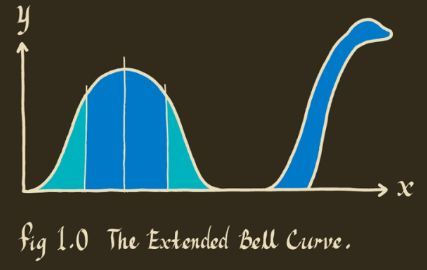
\includegraphics[width=4in, height=2.53in]{bellcurve.jpg}
\end{figure}
\FloatBarrier

\problem We will look at applications of the Central Limit Theorem (CLT).

\benum
\easysubproblem State the CLT for $\Xbar$ using the $\mu, \sigma$ notation. Be as complete as you can.
\easysubproblem Assume $\Xoneton \iid \bernoulli{p}$. State the CLT for $\hat{P}$ using the notation from class. Explain why we use the $\hat{P}$ notation and not the usual $\Xbar$ notation.
\intermediatesubproblem You randomly sample 100 people in an apartment building. Assume the population as a whole has equal distribution of males and females. What is the probability more than 60 people are male? Assume this sample is an SRS with respect to gender.
\intermediatesubproblem In homework \#2 problem 3 (a), you created a r.v. for the outcome of a \$5 American Roulette bet on black. Find the probability after 30 bets you come out ahead.
\hardsubproblem Assume the same configuration in the previous problem. Find the probability after 40 bets you lose more than 30 cents \textit{on average}.
\extracreditsubproblem Find a quote of beauty about the CLT that is different from the one in class. Write down the quotation, where you got it from, who said it (whether it's apocryphal or not), and the year.
\eenum

\problem We will now examine how quickly the CLT converges for the binomial r.v. with different $n,p$. Download the file \texttt{binomial\_clt.txt} from the webcafe portal and open it with a text editor. Copy all the code into \texttt{R} and press enter. This may take your computer 5 full minutes to compute, please be patient. You will now see a large plot. Each row of the plot represents the following random variables indexed by row number:

\beqn
X_{\text{row 1}} &\sim& \bernoulli{0.5} \\
X_{\text{row 2}} &\sim& \bernoulli{0.1} \\
X_{\text{row 3}} &\sim& \bernoulli{0.01} \\
X_{\text{row 4}} &\sim& \bernoulli{0.001} \\
\eeqn

Therefore, the row varies $p$. The six columns vary $n$, representing different sample sizes: $n=5, 10, 100, 1000, 10000, 100000$. The plots are the histogram estimates of the PMF's $S_n$ (the sum of $n$ for each of the different r.v.'s). 

\benum
\easysubproblem Maximize the plot window so you can examine it as closely as possible. At what $n$ for each of these Bernoulli's does its $S_n$ distribution approach the normal density \ie appear bell-like in the plot window? Phrased equivalently: at what $n$ does the binomial ``look'' normal?
\intermediatesubproblem We learned about the two sample size conditions for the normal approximation to the binomial in class as Rule 1: $np > 10$ and Rule 2: $n(1-p) > 10$. Below are the values of each of these calculations:

\begin{table}[htp]
\centering
\begin{tabular}{c|cccccc}
$p \downarrow, n \rightarrow$	&5	&10	&100	&1000&	10000&	1000000 \\
\hline
0.5	&2.5	&5	&50	&500	&5000	&500000 \\
0.1	&0.5	&1	&10	&100	&1000	&100000 \\
0.01	&0.05	&0.1	&1 &	10	&100	&10000 \\
0.001&	0.005	&0.01	&0.1	&1	&10	&1000 \\
\end{tabular}
\label{tab:authorship}
\caption{Calculation of $np$}
\end{table}
\FloatBarrier

\begin{table}[htp]
\centering
\begin{tabular}{c|cccccc}
$p \downarrow, n \rightarrow$	&5	&10	&100	&1000&	10000&	1000000 \\
\hline
0.5	&2.5	&5	&50	&500	&5000	&500000 \\
0.1	&4.5	&9	&90	&900	&9000	&900000 \\
0.01	&4.95	&9.9	&99	&990	&9900	&990000 \\
0.001&	4.995	&9.99	&99.9	&999	&9990	&999000 \\
\end{tabular}
\label{tab:authorship}
\caption{Calculation of $n(1-p)$}
\end{table}
\FloatBarrier

For each Bernoulli, what is the minimum $n$ that satisfies \textit{both} conditions? Is your answer the same as part (a) when you visually inspected the plots?

\easysubproblem Sum up what you've learned: when can we use the normal table to approximate the binomial?
\hardsubproblem Let's say $X_1, \ldots, X_{100} \iid \bernoulli{40\%}$. Calculate the probability of 39 successes out of 100 using the normal approximation. Compare it to the exact probability computed via the binomial PMF. This is \textit{really} hard and it's not extra credit because I want you all to attempt it. Do this one at the end of the assignment.
\eenum

\paragraph{Control Theory} These questions will get your feet wet with the concepts in chapter 14. \\

\problem We will learn about the two types of errors.

\benum
\easysubproblem What is the symbol we use for Type I errors? Make a probability statement using this symbol.
\easysubproblem Let's say you have a fire alarm in the building. The fire alarm can be ``off'' or ``on'' and there's either a ``fire'' or ``no fire''. Draw a $2 \times 2$ matrix like the one in class (table 14.2 on p.332) and indicate clearly what the row axis represents, what the column axis represents, and the labels for the rows and columns.
\easysubproblem Explain what a Type I error would be in the building / fire example without using technical jargon. 
\easysubproblem What is the cost of a Type I error?
\easysubproblem Explain what a Type II error would be in the building / fire example without using technical jargon.
\easysubproblem What is the cost of a Type II error?
\intermediatesubproblem You are the casino manager at Harrah's in Las Vegas. You are concerned about your Roulette wheels landing on black too often. You want to use the tools of ch 14 to track this potential problem. ``Shutdown'' would be shutting down the roulette tables. In fact, you want to duplicate exactly the statistical methodology that the book uses to look at computer chip HALT scores. Draw a mock control chart. Indicates axes and make up control limits. Do not do any calculations. This is purely a conceptual and visual problem.
\intermediatesubproblem How can the casino manager make a Type I error?
\intermediatesubproblem How can the casino manager make a Type II error?
\eenum
\end{document}
